\documentclass[tikz]{standalone}

\usepackage{tikz}
\usetikzlibrary{trees}
\usetikzlibrary{shapes}
\usetikzlibrary{positioning}
\usetikzlibrary{arrows.meta}

\tikzset{
    pointer/.style = {thick,draw=black,triangle 45-*,shorten >=-3pt},
    cell/.style = {rectangle, thick, draw=black,minimum width = 1cm, minimum height =1.0cm,fill=yellow!20},
    mynode/.style = {circle, thick, draw=black, align=center,fill=yellow!40,font=\ttfamily\bfseries\Large},
    mynoder/.style = {circle, thick, draw=black, align=center,fill=red!30,font=\ttfamily\bfseries\Large},
    mynodeb/.style = {circle, thick, draw=black, align=center,fill=blue!30,font=\ttfamily\bfseries\Large},
    edgen/.style = {-latex,ultra thick},
    edger/.style = {-latex,ultra thick,red},
    edgeb/.style = {-latex,ultra thick,blue},
    edgeg/.style = {-latex,ultra thick,gray},
    edgegd/.style = {-latex,ultra thick,brown,dashed}, % back
    edgevd/.style = {-latex,ultra thick,violet,dotted}, % forward
    edgexd/.style = {-latex,ultra thick,blue,densely dotted}, % traversal
    every picture/.style={/utils/exec={\ttfamily\bfseries}},
    every picture/.style={font issue=\ttfamily\bfseries},
    font issue/.style={execute at begin picture={#1\selectfont}
  }
}

\newcommand{\R}[1]{\textcolor{red}{#1}}
\newcommand{\B}[1]{\textcolor{blue}{#1}}
\newcommand{\G}[1]{\textcolor{violet}{#1}}

\begin{document}

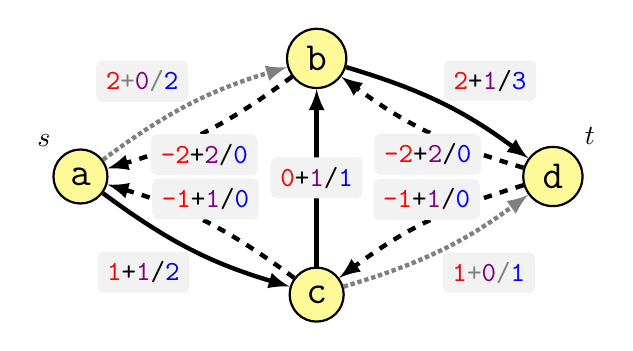
\begin{tikzpicture}[scale=1.00,transform shape]
\node[mynode, label={above left:$s$}] at (0.0, 1.5) (a) {a};
\node[mynode] at (3.0, 3.0) (b) {b};
\node[mynode] at (3.0, 0.0) (c) {c};
\node[mynode, label={above right:$t$}] at (6.0, 1.5) (d) {d};
\draw[edgen,gray,densely dotted] (a) edge[bend left=10, above left] node[rounded corners=2pt,fill=gray!10] {\R{2}+\G{0}/\B{2}} (b);
\draw[edgen] (b) edge[dashed,bend left=10, below] node[rounded corners=2pt,fill=gray!10] {\R{-2}+\G{2}/\B{0}} (a);
\draw[edgen] (a) edge[bend right=10, below left] node[rounded corners=2pt,fill=gray!10] {\R{1}+\G{1}/\B{2}} (c);
\draw[edgen] (c) edge[dashed,bend right=10, above] node[rounded corners=2pt,fill=gray!10] {\R{-1}+\G{1}/\B{0}} (a);
\draw[edgen] (c) edge node[rounded corners=2pt,fill=gray!10] {\R{0}+\G{1}/\B{1}} (b);
\draw[edgen,gray,densely dotted] (c) edge[bend right=10, below right] node[rounded corners=2pt,fill=gray!10] {\R{1}+\G{0}/\B{1}} (d);
\draw[edgen] (d) edge[dashed,bend right=10, above] node[rounded corners=2pt,fill=gray!10] {\R{-1}+\G{1}/\B{0}} (c);
\draw[edgen] (b) edge[bend left=10, above right] node[rounded corners=2pt,fill=gray!10] {\R{2}+\G{1}/\B{3}} (d);
\draw[edgen] (d) edge[dashed,bend left=10, below] node[rounded corners=2pt,fill=gray!10] {\R{-2}+\G{2}/\B{0}} (b);
\end{tikzpicture}


\end{document}